\input{../common/header}

\begin{document}

\lecture{ 27 --- File System Implementation and Allocation Methods }{\term}{Jeff Zarnett}

\subsection*{File System Implementation}

We mentioned earlier that there are a lot of different file systems, like ext3, ZFS, etc. These may co-exist in the same system, though a partition will be formatted in only one of them. From the user's perspective, however, these operate identically. This is because of an additional layer of abstraction, called the virtual file system (VFS). 

There are two main purposes to the VFS. The first is to separate the file system operations (like reading, writing, opening, and closing files) from the actual implementation; thus operations can be done with whatever file system is actually implemented. The second is that it provides a mechanism for representing a file, uniquely, throughout a network. The file representation structure is called a \textit{vnode}, which is rather like an inode, but inodes are unique only within one file system. The VFS distinguishes between local and remote files~\cite{osc}.

\begin{center}
	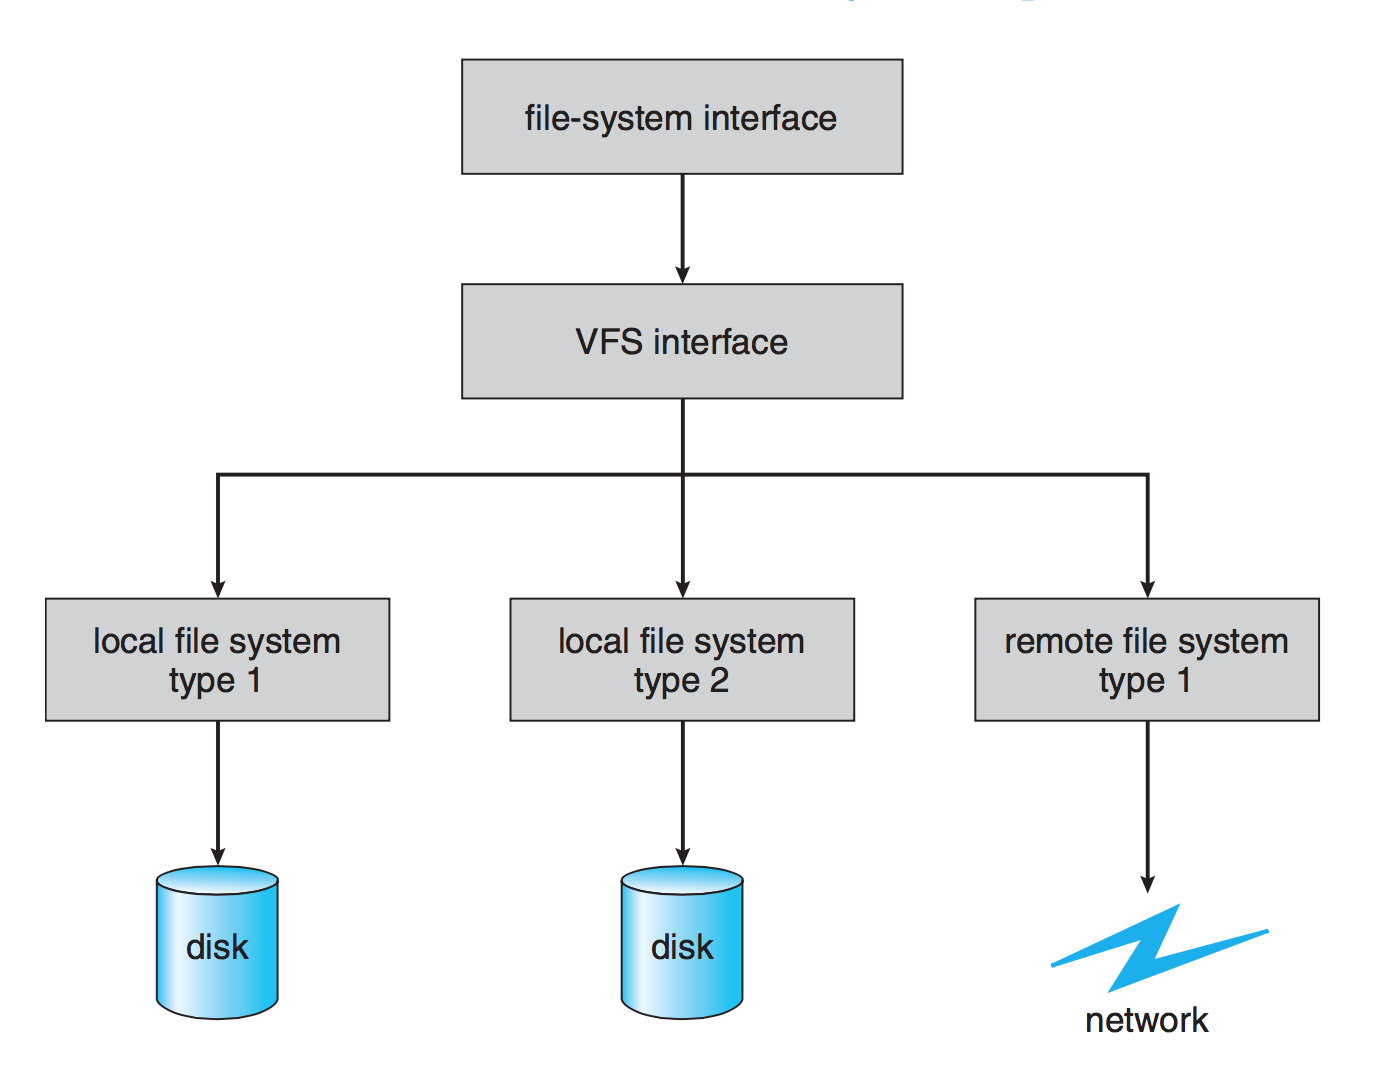
\includegraphics[width=0.5\textwidth]{images/vfs.png}\\
	Schematic view of the VFS Interface~\cite{osc}.
\end{center}

The VFS architecture in Linux has four main objects~\cite{osc}:
\begin{enumerate}
	\item inode (an individual file)
	\item file (an open file)
	\item superblock (the file system)
	\item dentry (a directory entry)
\end{enumerate}

For each of those, there are a set of operations defined. In the Linux kernel, these operations are defined in the \texttt{fs.h} headers and may include functions such as:

\begin{verbatim}
 ssize_t (*read) (struct file *, char __user *, size_t, loff_t *);
 ssize_t (*write) (struct file *, const char __user *, size_t, loff_t *);
 int (*open) (struct inode *, struct file *);
 int (*flush) (struct file *, fl_owner_t id);
 int (*release) (struct inode *, struct file *);
\end{verbatim}

The VFS therefore abstracts away a lot of the details of the underlying file system implementation.

\subsection*{Directory Implementation} 

See the table below for some information about what data may appear in a typical file directory. This is just to show that directories are much more complicated than we're going to talk about in this course.

\begin{center}
	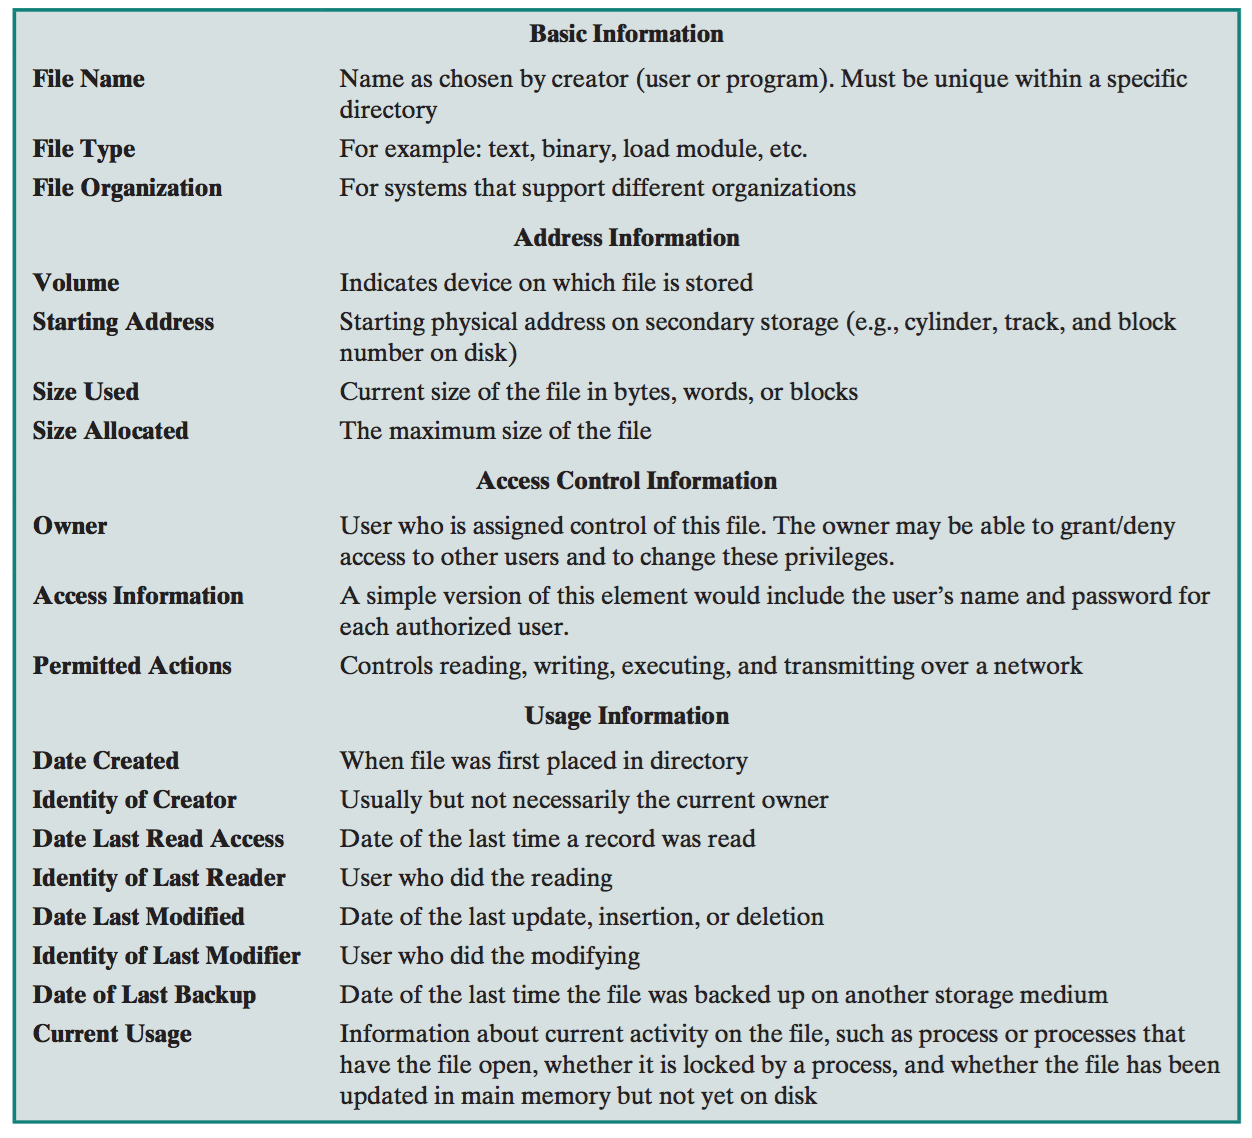
\includegraphics[width=0.75\textwidth]{images/directory.png}\\
	Information elements of a file directory~\cite{osi}.
\end{center}

The simplest version of a directory is what we'll talk about and that's just a set of files. And yet, there is a choice to be made in implementing them: a linear list versus a hash table. Both concepts should be familiar to you from data structures and algorithms.

The linear list option is certainly the simplest. Creating a new file requires searching the directory to see if there is a matching file name. If not, insert that new entry in the list. Deletion is also simple: search the list for the matching file and remove it; if it is the last reference to that file, we can free up the space. The real disadvantage to linear lists is that searching takes a long time. Searching through a directory can take quite a while, and the problem is compounded if the search is supposed to include the content of the file as well.

Alternatively, we could use a hash table. The hash is computed based on the file name, and of course there will need to be some strategy for dealing with hash collisions. Still, neither of these is satisfactory; what we really want is a more complex structure: a tree.

An AVL tree might be good as a way of storing ordered data, but it does not match well with the block system of a hard drive. Instead, we will examine a B-Tree, a variation on a binary search tree. 

Each node should occupy one block, so each node can contain a lot of information. File and directory information is linearly ordered, but a block does not need to be full. If a leaf node gets full, we can split it into two half-full blocks. Keeping the tree balanced means it takes about the same amount of time to find an item wherever it is.

A B-Tree structure, formally, has the following characteristics~\cite{osi}:

\begin{enumerate}
	\item The tree is made up of nodes (have children) and leaves (have no children).
	\item Each node contains at least one key identifying a file record, and more than one pointer to child nodes or child leaves.
	\item Each node has some maximum number of keys.
	\item The keys in a node are stored in non-decreasing order.
\end{enumerate}

And a B-tree of degree $d$ has the following properties~\cite{osi}:

\begin{enumerate}
	\item Every node has at most $2d-1$ keys and $2d$ children ($2d$ pointers).
	\item Every node other than the root has at least $d-1$ keys and $d$ pointers. Each internal node except the root is at least half full and has at least $d$ children.
	\item All leaves appear on the same level.
	\item A non-leaf node with $k$ pointers contains $k-1$ keys.
\end{enumerate}

To find something in a B-Tree, the general algorithm is fairly simple~\cite{osi}:

\begin{enumerate}
	\item Start at the root node. 
	\item If the key is in the current node, it is found, and the algorithm terminates.
	\item If the key is less than the smallest key in this node, follow the leftmost pointer; go to step 2.
	\item If the key is greater than the largest key in this node, follow the rightmost pointer; go to step 2.
	\item If the key is between the values of two adjacent keys, follow the pointer between them; go to step 2.
\end{enumerate}


Insertion into the B-Tree is more complicated, because of the rules that keep the tree balanced~\cite{osi}:

\begin{enumerate}
	\item Search the tree for the key. If it is not found, then we are at least looking at the block where it would be if it were there.
	\item If this node has fewer than $2d-1$ keys (that is, it is not full), insert the key into this node in the proper sequence. The algorithm terminates.
	\item If the node is full, split this node around the median key into two new nodes with $d-1$ keys each. Promote the median key to the higher level. If the new node is less than the median key, insert it in the left-hand new node; otherwise into the right.
	\item The promoted node is inserted into the parent node in order, splitting the parent if the parent is already full.
	\item If the process of promotion reaches the root node and the root is full, then splitting and promotion occurs and the height of the tree increases by 1.
\end{enumerate}

Some examples of how the insertion algorithm runs are shown below:

\begin{center}
	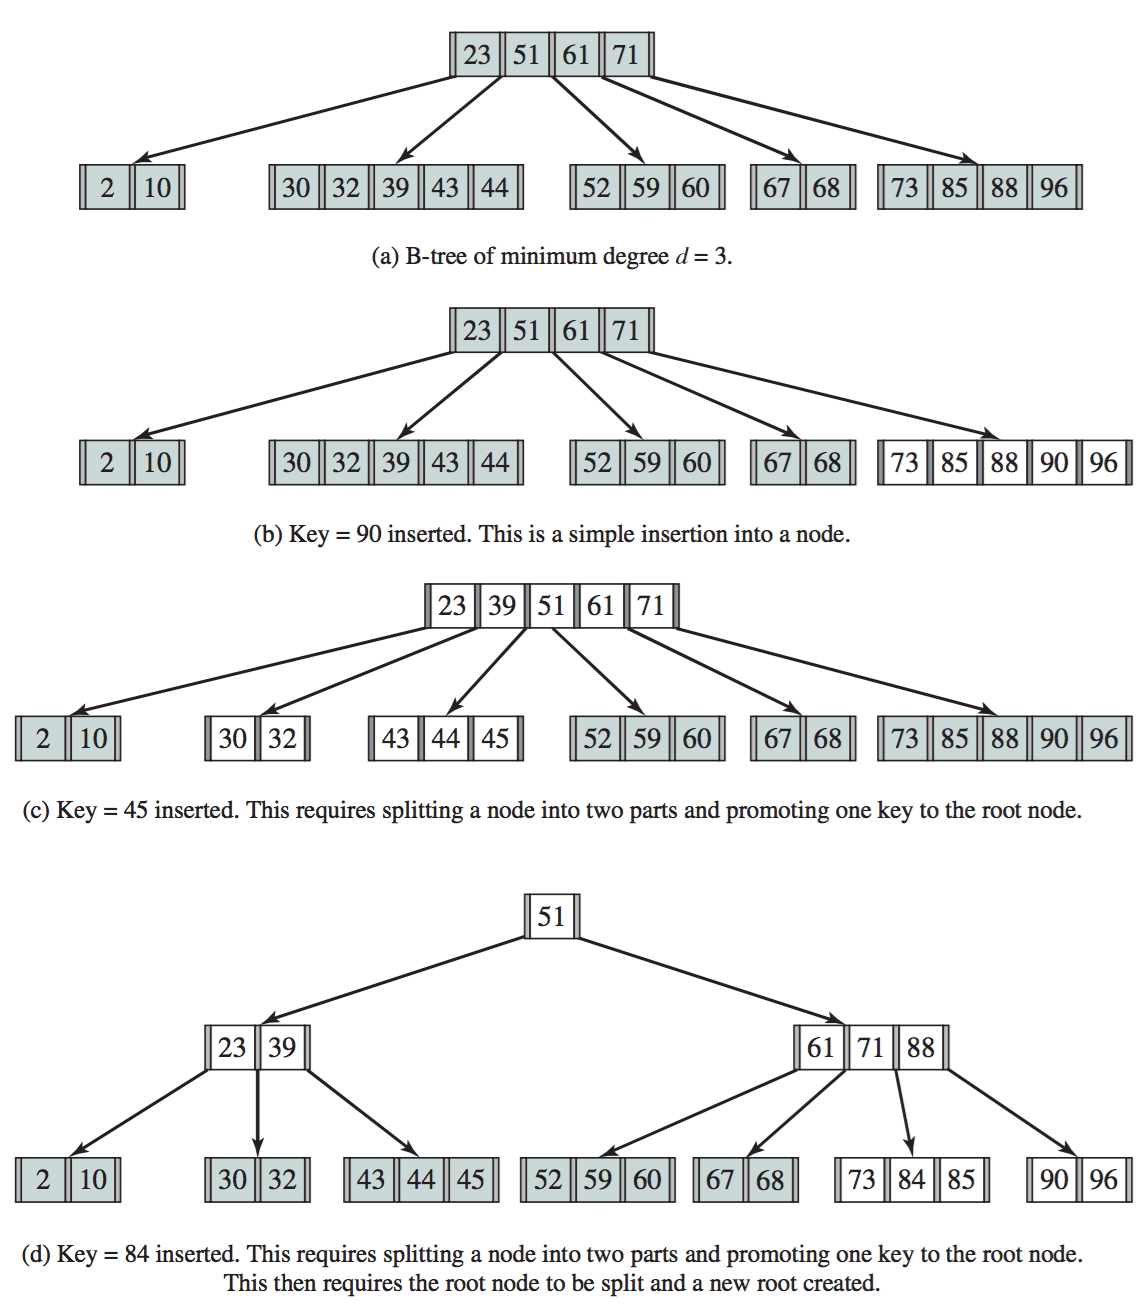
\includegraphics[width=0.9\textwidth]{images/b-tree-insert.png}\\
	Insertion of nodes 90, 45, and 84 into a B-Tree~\cite{osi}.
\end{center}

\section*{File Allocation Methods}

Much like memory allocation, there is a need to choose a strategy for how to allocate disk space. There are three major ways that we could allocate the disk space to files: contiguous, linked, and indexed; each has its advantages and disadvantages.

\subsection*{Contiguous Allocation}
The contiguous allocation strategy means that a file occupies a set of contiguous blocks on disk. So a file is allocated, starting at block $b$ and is $n$ blocks in size, the file takes up blocks $b, b+1, b+2, ..., b+(n-1)$. This is advantageous, because if we want to access block $b$ on disk, accessing $b+1$ requires no head movement, so seek time is nonexistent to minimal (if we need to move to another cylinder). 

All that we need to maintain are the values of $b$ and $n$: the start location and length of the file. Both sequential and direct access are very easy: the first block of a file is at $b$. To access a block $i$ at some offset into the file, it is simply at the base address $b$ plus $i$. Checking if the access is valid is also an easy operation: if $i < n$ then it is valid.

See the diagram below to get an example of contiguous allocation:
\begin{center}
	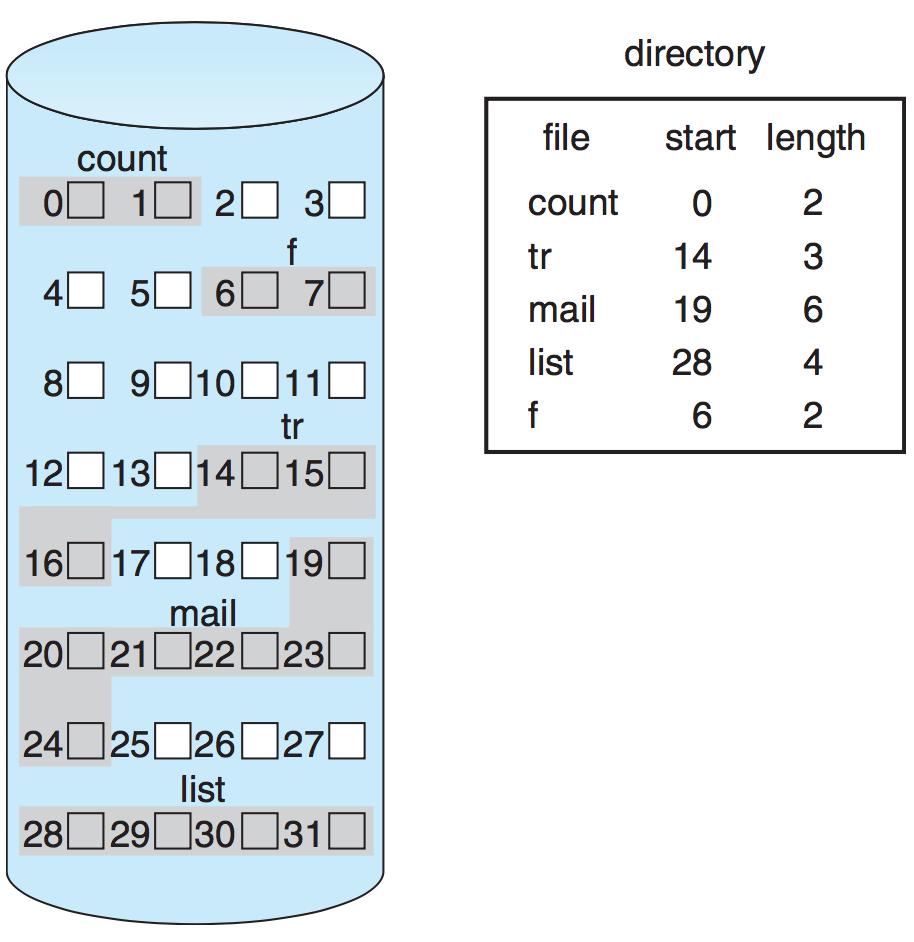
\includegraphics[width=0.4\textwidth]{images/disk-contiguous.png}\\
	Contiguous allocation of disk space~\cite{osc}.
\end{center}

This takes us back to a problem we have seen once before: the memory allocation problem. If we need a memory block of size $N$: (1) can we find a contiguous block of $N$ or greater to meet that allocation? and (2) if there is more than one block, which one do we choose? As before, we suffer the problem of external fragmentation, plus a bit of internal fragmentation in the last block of the file. 

There was also talk on the subject of memory allocation of compaction. This was moving memory allocations around in memory to create some larger free spaces that can be allocated. But for languages like C, it was not realistic, because of the impossibility of updating all pointers (unlike Java where we can update all references). We can do compaction on disk, but it takes a very, very long time and is computationally expensive. Doing compaction can be done when the system has nothing else to do (idle priority operation) or on some schedule when it would be minimally disruptive (e.g., middle of the night... mind you... a lot of programmers do most of their work in the middle of the night...).

Another problem, of course, with contiguous allocation is that old clairvoyance issue: how much space is a file going to take? If it is just a copy-paste operation, the copy is the same size as the original, so there is no problem. When a user opens a new document, how does the OS know how big the file is going to be? Is this a 3 page essay or a 300 page thesis? If we allocate too little space, we may be able to tack on space at the end, or that block may be allocated, forcing us to move the file and reallocate it. If the value we choose is too large, then significant space will be wasted for small files (and many files tend to be relatively small)~\cite{osc}. 

\subsection*{Linked Allocation}
Linked allocation is a solution to the problems of contiguous allocation: instead of a file being all in consecutive blocks, we maintain a linked list of the blocks, and the blocks themselves may be located anywhere on the disk. The directory listing just has a pointer to the first and last blocks (head and tail of the linked list).

If a new file is created, it will be created with size zero and the head and tail pointers are null. When a new block is needed, it can come from anywhere and will just be added to the linked list. Thus, compaction and relocation are not really an issue. Unfortunately, however, accessing block $i$ of a file is no longer as simple as computing an offset from the first block; it requires following $i$ pointers (a pain).

\begin{center}
	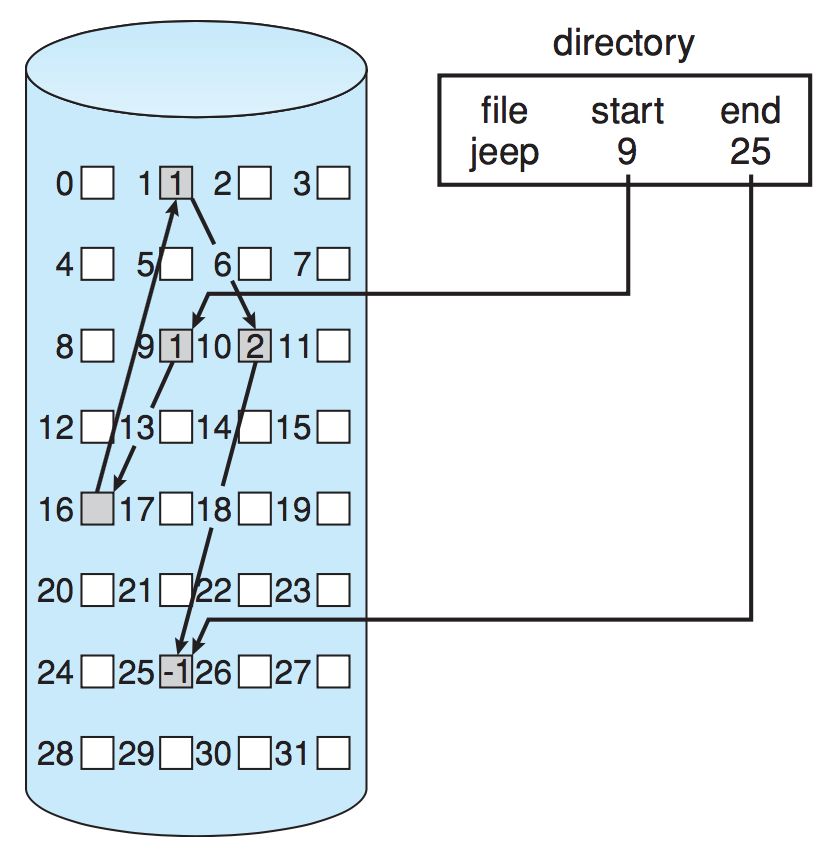
\includegraphics[width=0.4\textwidth]{images/disk-linked.png}\\
	Linked allocation of disk space~\cite{osc}.
\end{center}

A possible solution to the problem of following so many pointers (and the overhead of maintaining so many) is to group up the blocks into \textit{clusters}, where a cluster is comprised of, say, four blocks. Then we waste less memory maintaining pointers and it improves disk accesses because there is less seeking back and forth to various disk locations~\cite{osc}. 

One variation of linked allocation is the File Allocation Table (FAT), which was used by the MS-DOS operating system (FAT16 and FAT32 were used in Windows before NTFS came in with NT/2000/XP and their descendants). The FAT32 file system hangs on these days as the file system of choice for formatting USB flash drives because it means the data will be readable in Windows, Mac OS X, and Linux. This is primarily because Microsoft has not made the NTFS file system standard public and Windows systems do not support too many other file systems, and Windows has such a big marketshare. So the FAT32 option is used, despite its known problems (and limitations, like 4~GB max file size), because it's the one system everyone can understand. Isn't the state of personal computing so... uplifting?

The FAT allocation scheme works like this: at the beginning of the disk, there is a table to maintain file allocation data (hence the name). The table has one entry for each block and is indexed by block number. It works like a linked list; the directory entry has the first block of the file and the table entry under that block number has the index of the next block. The chain continues until the last block where there is a special end-of-file value. An unused block has a table value of 0. Thus, to allocate a new block, find the first 0-valued entry, and replace the previous end-of-file value with the address of the new block~\cite{osc}. See the example below:


\begin{center}
	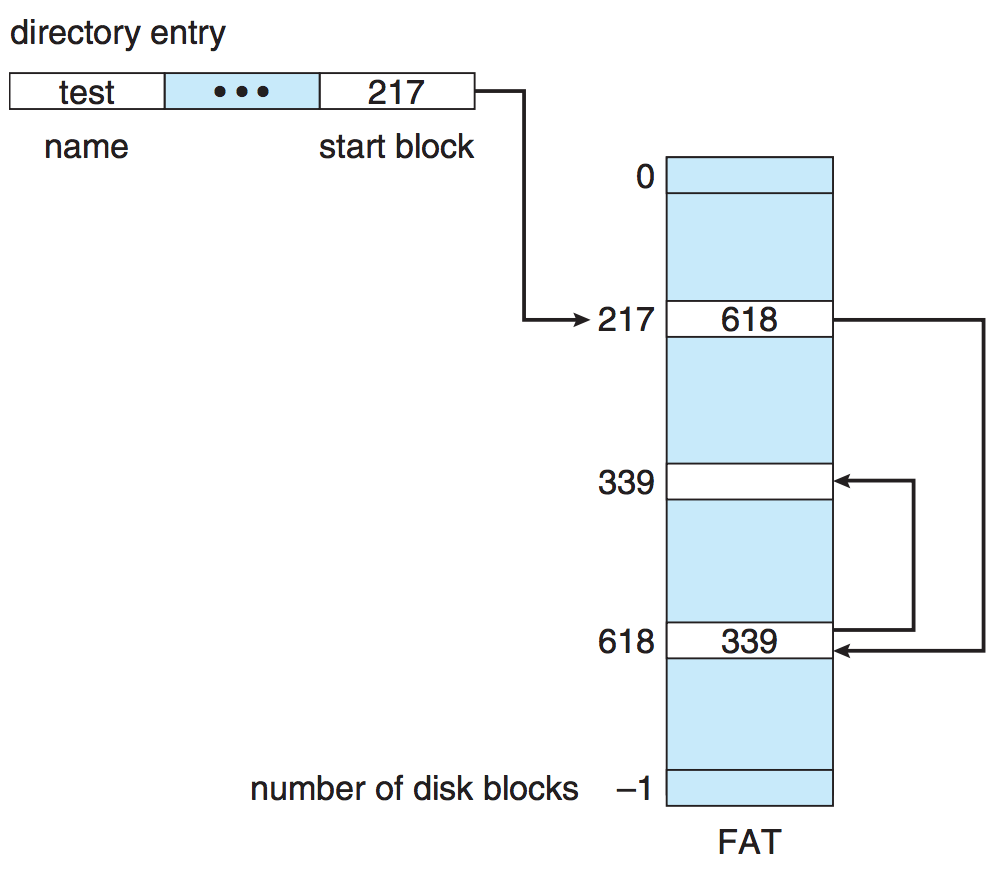
\includegraphics[width=0.5\textwidth]{images/file-allocation-table.png}\\
	File Allocation Table (FAT)~\cite{osc}.
\end{center}

The FAT itself should be cached in memory, otherwise the disk is going to have to seek back to it unbearably often.

\subsection*{Indexed Allocation}
If we stuck to pure linked allocation, we still have the problem that accessing some part in the middle of the file is a pain because we have to follow and retrieve a lot of pointers to the different blocks. The idea of indexed allocation is to take all the pointers and put them into one location: an index block. So, the first block of the file contains a whole bunch of pointers. To get to block $i$, just go to index $i$ of the index block and we can get the location of block $i$ much more efficiently than we could in linked allocation. All pointers to blocks start as null, and when we add a new block, add its corresponding entry into the index block~\cite{osc}. See the diagram below:

\begin{center}
	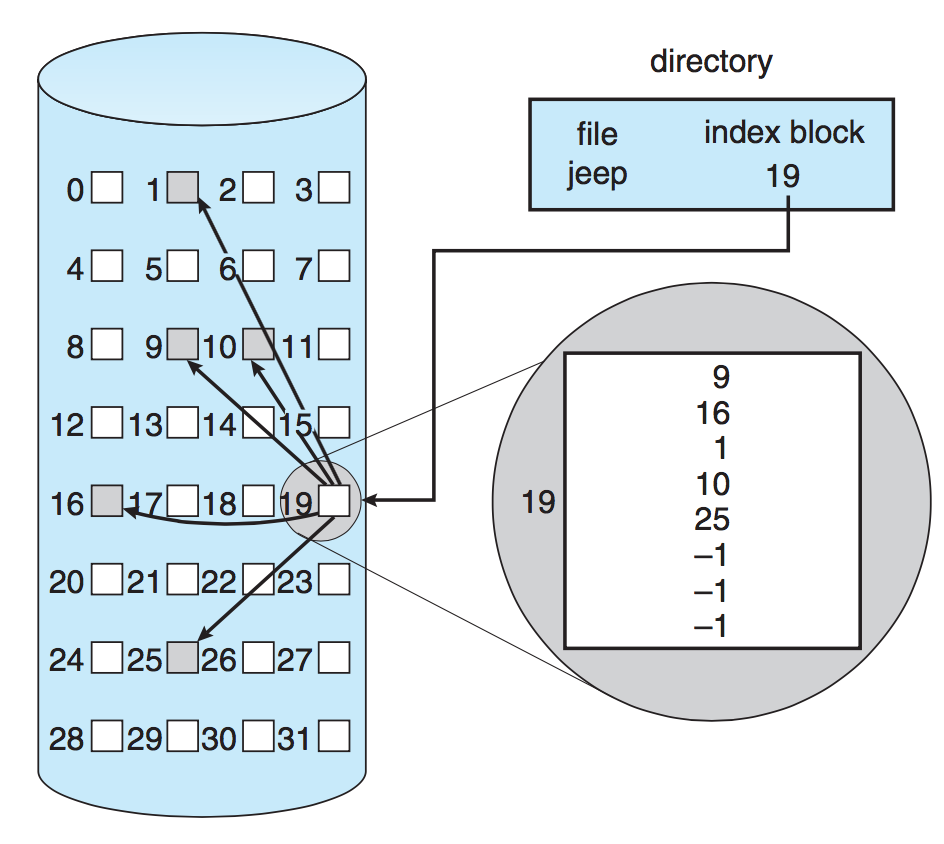
\includegraphics[width=0.4\textwidth]{images/disk-indexed.png}\\
	Indexed allocation of disk space~\cite{osc}.
\end{center}

Like many of the other systems we have examined, there is a need to make a decision about the size of a block. If a file needs only 1-2 blocks, one whole block is allocated for the pointers which contains only 1-2 entries. That suggests we want the index to be small, but what if we need more pointers than fit into one block? There are a few mechanisms for this~\cite{osc}:

\begin{enumerate}
	\item \textbf{Linked Scheme}: An index block is a disk block, and we can link together several index blocks. The last entry in the index block is either null or a pointer to the next index block.
	\item \textbf{Multilevel Index}: A variant of the linked scheme that has multiple levels. The first level block points to the second level block; the second level block points to the actual file data. This can go to as many levels are necessary based on the maximum file size. If a block is 4~KB, we can have 1024 4-byte pointers, so two levels would allow a maximum file size of up to 4~GB.
	\item \textbf{Combined Scheme}: The all-of-the-above option. This is used in UNIX. Keep the first 15 pointers of the index block in the inode structure; 12 of them point directly to file data. The next three pointers refer to indirect blocks. The 13th is an index block containing the addresses of blocks with data. The 14th points to a double indirect block (addresses of blocks containing addresses of blocks). The 15th points to a triple indirect block\footnote{Yo dawg, we heard you like index blocks...}.
\end{enumerate}

With that out of the way, we can finally show a visual representation of an inode.

\begin{center}
	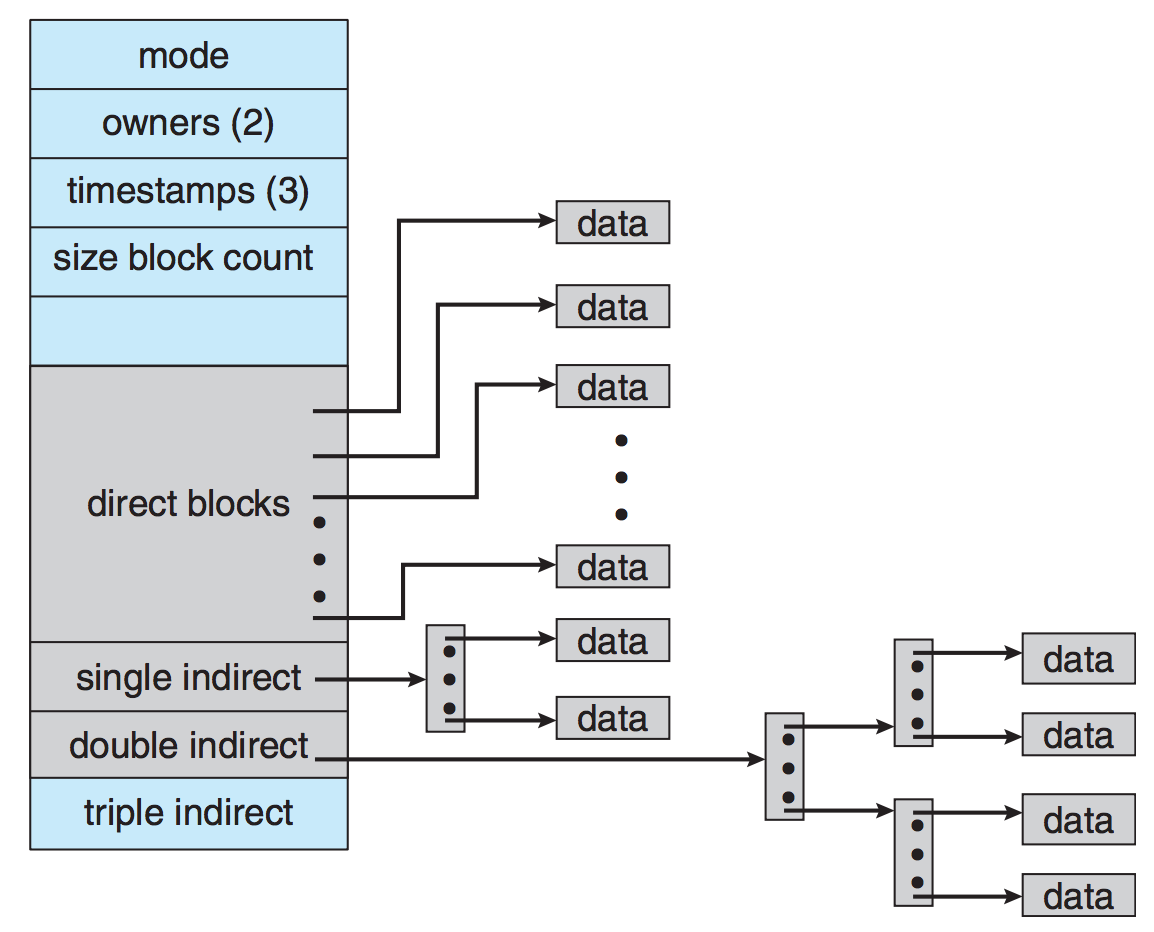
\includegraphics[width=0.6\textwidth]{images/unix-inode.png}\\
	The UNIX inode. Triple indirection is left to the reader's imagination~\cite{osc}.
\end{center}

\subsection*{Other Disk Issues}
As with memory, the system will keep track of the free space available.

Bit vectors work just the way we would expect: create a structure in memory where a bit represents a block. If it is free, the bit is 1; allocated is 0. So a bit vector looks like \texttt{0100110111011111000000...}. The problem with this strategy is, of course, that the bigger the disk, the more overhead is needed to store this bit vector.

The next rather obvious approach is a linked list: the head points to the first free space block, and we can traverse the list to get to the next free block. See the diagram below:

\begin{center}
	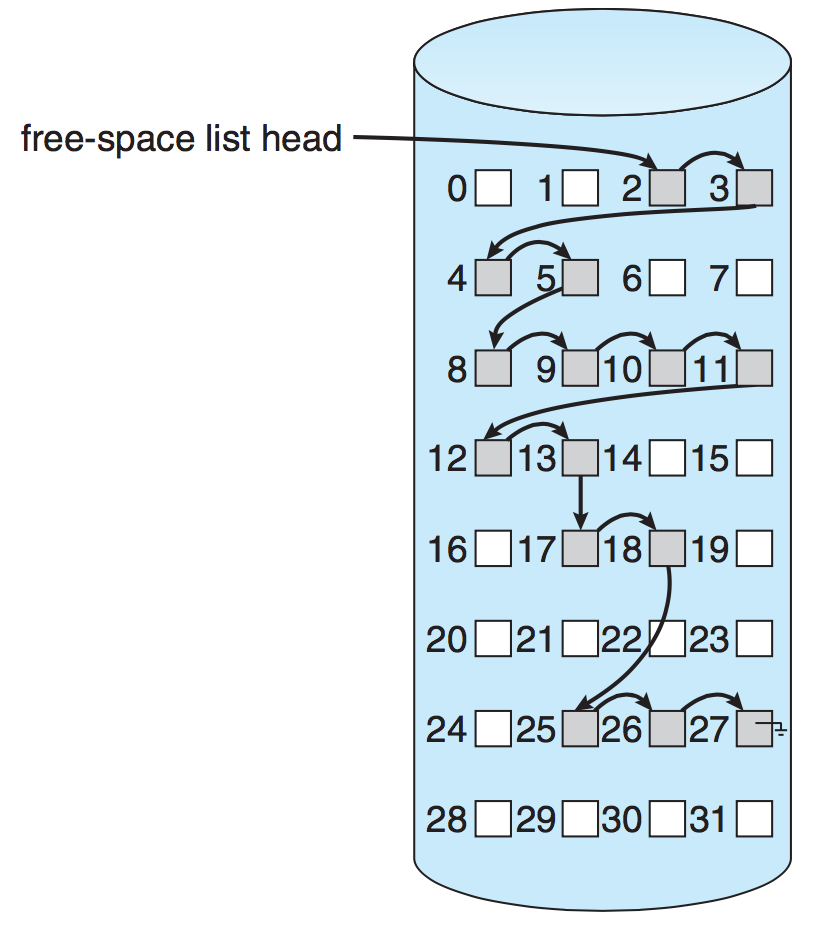
\includegraphics[width=0.4\textwidth]{images/disk-linked-list.png}\\
	Linked free-space list on disk~\cite{osc}.
\end{center}

Grouping makes this slightly more interesting: the first free block will be used to store the addresses of $n$ free blocks, the first $n-1$ of which are actually free. The last block contains a block with another set of $n$ free blocks. So if we need a large number of free blocks, we can find them quickly, instead of walking through the list one block at a time, which takes a lot of disk accesses. Counting is a slight improvement on this where we also store a number $k$ of free contiguous blocks after each address. So, if block 27 is followed by three consecutive free blocks, instead of having 27, 28, 29, 30 as entries, it will show (27, 4). The entries may be stored in a balanced tree for efficient operations~\cite{osc}.


The efficient use of a disk depends on the disk-allocation and directory algorithms. UNIX inodes, for example, are preallocated, so even a disk containing no files has some of its space taken up by the inodes. Preallocation of inodes and distribution of them improves the file system performance, because the UNIX allocation and free-space algorithms keep the file data near the inode, where possible, to reduce seek time~\cite{osc}.


\input{bibliography.tex}

\end{document}